\documentclass[conference]{IEEEtran}

\usepackage[margin=1in]{geometry}
\usepackage{setspace}
\usepackage{lmodern}
\usepackage[T1]{fontenc}
\usepackage[utf8]{inputenc}
\usepackage{microtype}
\usepackage{amsmath,amssymb}
\usepackage{booktabs}
\usepackage{tabularx}
\usepackage{array}
\usepackage{enumitem}
\usepackage{xcolor}
\usepackage{fancyhdr}
\usepackage{listings}
\usepackage{graphicx}
\usepackage[hidelinks]{hyperref}
\usepackage{titlesec}

\setstretch{1.15}
\setlist[itemize]{topsep=0.35em,itemsep=0.2em,leftmargin=1.4em}
\setlist[enumerate]{topsep=0.35em,itemsep=0.25em,leftmargin=1.6em}

\titleformat{\section}{\large\bfseries\raggedright}{\thesection.}{0.6em}{}
\titleformat{\subsection}{\normalsize\bfseries\raggedright}{\thesubsection.}{0.55em}{}
\titlespacing*{\section}{0pt}{1.15em}{0.45em}
\titlespacing*{\subsection}{0pt}{0.9em}{0.3em}

\lstset{
  basicstyle=\ttfamily\footnotesize,
  breaklines=true,
  frame=single,
  rulecolor=\color{black!40},
  columns=fullflexible,
  keepspaces=true,
  aboveskip=0.7em,
  belowskip=0.7em,
  showstringspaces=false
}

\pagestyle{fancy}
\fancyhf{}
\fancyhead[L]{\small PS-5 Mini-Project Report}
\fancyhead[R]{\small Scalable Parallel K-Means}
\fancyfoot[C]{\thepage}
\renewcommand{\headrulewidth}{0.4pt}
\setlength{\headheight}{14.5pt}
\graphicspath{{./}}

\hypersetup{
  pdftitle={Scalable Parallel K-Means Clustering Using MPI and CUDA},
  pdfauthor={Tirth Miteshkumar Patel, Aarush Arora, and Udit Asthana},
  pdfsubject={Parallel Computer Architecture and Programming (PS-5), Mini-Project Report}
}

\makeatletter
\newcommand{\forcelabel}[1]{\def\@currentlabel{#1}}
\makeatother
\DeclareRobustCommand{\code}[1]{\texttt{#1}}
\DeclareRobustCommand{\file}[1]{\texttt{#1}}

\begin{document}

% ------------------------------------------------------------------
% Full-width front matter; the remaining report stays two-column.
\twocolumn[{%
\begin{minipage}{\textwidth}
{\centering
{\large Parallel Computer Architecture \& Programming}\\[0.25em]
{\large Problem Statement 5}\\[1.15em]
{\LARGE\bfseries Scalable Parallel K-Means Clustering\\[0.2em]
Using MPI and CUDA}\\[1.05em]
{\Large Mini-Project Report}\\[0.9em]
\par}

\vspace{0.7em}
\noindent
This report compares three implementations of K-means on a synthetic dataset containing 100,000 points and 16 features. The serial CPU program provides the reference result. The MPI version divides the points between two ranks, while the hybrid version uses MPI for distributed work and CUDA for the local point-assignment step.

\vspace{0.85em}
\centering
\renewcommand{\arraystretch}{1.25}
\begin{tabularx}{\textwidth}{@{}l X@{}}
\toprule
\textbf{Field} & \textbf{Detail} \\
\midrule
Course & Parallel Computer Architecture \& Programming (PS-5) \\
Problem statement & Scalable parallel clustering for large point sets \\
Project title & Scalable Parallel K-Means Clustering Using MPI and CUDA \\
\bottomrule
\end{tabularx}

\vspace{0.75em}
\raggedright
\noindent\textbf{Team}

\vspace{0.35em}
\noindent\textbf{1. Tirth Miteshkumar Patel} \quad Reg.\ 240905272 \quad Roll 27 \quad CSE D\\
Distributed-memory MPI design, dataset partitioning, synchronization, scaling analysis, and the shared numerical core.

\vspace{0.35em}
\noindent\textbf{2. Aarush Arora} \quad Reg.\ 240905266 \quad Roll 26 \quad CSE D\\
CUDA assignment kernel, device-side reduction, CPU fallback when no GPU is present.

\vspace{0.35em}
\noindent\textbf{3. Udit Asthana} \quad Reg.\ 240905310 \quad Roll 31 \quad CSE D\\
Integration of the MPI driver and the CUDA kernel into \code{kmeans\_hybrid}: the shared assignment contract, the \code{USE\_CUDA\_KERNEL} build, and the runners that validate the bound binary against the serial reference.
\end{minipage}
}]

\clearpage
\onecolumn
\tableofcontents
\clearpage
\twocolumn

% The figures are expected to be in the same folder as this .tex file.
% ------------------------------------------------------------------
\section{Abstract}
\label{sec:abstract}
K-means divides a dataset into $K$ clusters by repeatedly assigning each point to its nearest centroid and recalculating the centroids. The assignment phase requires $O(NKD)$ distance work per iteration, so it is the main target for parallel execution.

This project implements three versions of the algorithm: serial CPU, MPI CPU, and hybrid MPI+CUDA. The MPI program partitions the points across ranks and combines local cluster sums and counts with \code{MPI\_Allreduce}. In the hybrid version, a CUDA kernel performs the local assignment work when a usable GPU is available; the program falls back to the CPU path when it is not.

The benchmark uses $N=100{,}000$ data points, $D=16$ features, and $K=10$ clusters. The supplied plot summarizes 20 timing runs for each version. Mean runtime falls from 1.222 s for the serial program to 0.943 s for two-rank MPI and 0.621 s for the hybrid version. These results give mean speedups of about $1.30\times$ and $1.97\times$, respectively. They describe this workload and test environment; further runs at different process counts and data sizes are needed to assess scaling.

% ------------------------------------------------------------------
\section{Keywords}
\label{sec:keywords}
K-means clustering; high-performance computing; MPI; CUDA; distributed-memory parallelism; GPU acceleration; speedup; parallel efficiency; execution-time analysis.

% ------------------------------------------------------------------
\section{Introduction}
\label{sec:intro}
Each Lloyd iteration of K-means has two main stages. First, every point is assigned to the centroid with the smallest squared Euclidean distance. Second, each non-empty cluster's centroid is replaced by the mean of its assigned points. The assignment stage costs $O(NKD)$ per iteration, whereas the centroid update works on only $K$ clusters with $D$ coordinates each.

Point assignments are independent within an iteration, which makes them suitable for parallel execution. In the MPI version, each rank works on a separate block of points. The ranks then combine their local cluster sums and counts through a collective reduction. Since the reduction exchanges centroid statistics rather than the full point matrix, its data volume depends on $K$ and $D$, not directly on $N$.

The hybrid version applies the same idea within each rank: a CUDA kernel assigns local points to centroids, while MPI coordinates the distributed update. The measured runtime includes the work needed to allocate device buffers and transfer data, so the results reflect the full implementation rather than kernel execution alone.

% ------------------------------------------------------------------
\section{Literature Review}
\label{sec:literature}
MacQueen's early work described a method for classifying multivariate observations through repeated reassignment \cite{macqueen1967}. Lloyd later formalized the iterative least-squares procedure commonly used for K-means \cite{lloyd1982}. Both works underpin the assignment-and-update loop used in this project.

Distributed implementations divide the dataset among processes and combine their local statistics to update centroids. Dhillon and Modha examined clustering on distributed-memory multiprocessors and showed how this approach can be used for larger workloads \cite{dhillon2000}. The MPI implementation here follows the same general pattern: ranks retain their own points and exchange the sums and counts needed for the next iteration.

GPU-based K-means implementations parallelize the distance calculations for different points. Farivar et al. and Li et al. studied approaches to GPU execution and its associated performance costs \cite{farivar2008,li2013}. The hybrid version in this report uses CUDA for the assignment step and MPI for distributing points and combining cluster statistics. Results from those papers are useful context, but their hardware and test data differ from the present experiment, so their reported runtimes are not treated as a numerical baseline.

The implementation also supports K-means++ initialization, which chooses starting centroids with probabilities based on each point's distance from the selected centers \cite{arthur2007}. For correctness checks, centroid labels are matched by minimum cost because two valid K-means runs can number the same clusters differently.

% ------------------------------------------------------------------
\section{Problem Statement}
\label{sec:problem}
Problem Statement 5 requires a K-means program that can be run in serial, across MPI processes, and with GPU acceleration. The three versions need to use the same data format and centroid-update rule so that their results can be compared on a common basis.

The implementation follows four practical requirements:
\begin{itemize}
  \item The serial, MPI, and hybrid programs read the same binary input format.
  \item Rank 0 reads the complete point matrix and distributes contiguous blocks to the other ranks.
  \item Each iteration records computation and communication timing separately.
  \item The CUDA assignment routine follows the CPU routine's interface, allowing a CPU fallback when a usable GPU is unavailable.
\end{itemize}

The default stopping condition uses the largest centroid movement between consecutive iterations:
\[
  \Delta = \max_{k:\, n_k > 0}\big\|\mu_k^{\mathrm{new}} - \mu_k^{\mathrm{old}}\big\|_2 < \tau,
\]
where $\tau=10^{-4}$ and the iteration limit is 100.

% ------------------------------------------------------------------
\section{Objectives}
\label{sec:objectives}
The work was organized around the following objectives:
\begin{enumerate}
  \item Build serial CPU, MPI CPU, and hybrid MPI+CUDA versions around a shared numerical implementation.
  \item Test the versions on a synthetic workload with $N=100{,}000$, $D=16$, and $K=10$.
  \item Summarize 20 runtime measurements per mode using mean and median values.
  \item Calculate speedup against the serial baseline and estimate two-rank MPI efficiency.
  \item Check that parallel runs produce comparable SSE values and centroid sets.
  \item Present the measurements in plots and tables, with execution screenshots added from actual runs.
\end{enumerate}

% ------------------------------------------------------------------
\section{Proposed Methodology}
\label{sec:methodology}
The benchmark compares the three implementations on a synthetic matrix with 100,000 points and 16 features, using 10 clusters. The supplied performance plot contains 20 timing runs for each mode. Mean and median runtime are used because the mean reflects overall time while the median is less affected by occasional slow runs.

The serial CPU version provides the reference. The MPI CPU version divides the points between two ranks, assigns each rank's local points, and reduces the cluster sums and counts. In the hybrid version, the same distributed iteration calls a CUDA kernel for local point assignment when a compatible device is available. The measured hybrid time includes memory allocation, data transfers, kernel execution, synchronization, and copying results back to the host.

Correctness checks are kept separate from timing. The validation script compares the SSE objective and matches candidate centroids to the reference set using a minimum-cost assignment. This allows cluster identifiers to differ while still checking whether the resulting centroid sets agree. For reproducibility, raw results should also record the CPU and GPU models, compiler, MPI and CUDA versions, build flags, and random seed. Those details are not visible in the supplied plot and should be taken from the run logs.

% ------------------------------------------------------------------
\section{System Architecture}
\label{sec:architecture}

\begin{table*}[t]
\centering
\caption{Implementation variants and their assignment paths.}
\label{tab:binaries}
\renewcommand{\arraystretch}{1.2}
\begin{tabularx}{\textwidth}{@{}p{1.7in} p{1.25in} X@{}}
\toprule
\textbf{Binary} & \textbf{Build target} & \textbf{Assignment} \\
\midrule
\code{bin/kmeans\_serial}  & \code{make serial} & \code{assign\_points\_cpu} on all $N$ points \\
\code{bin/kmeans\_mpi}     & \code{make mpi}    & \code{assign\_points\_cpu} on the local block \\
\code{bin/kmeans\_hybrid}  & \code{make hybrid} & \code{launch\_assignment\_kernel} on the local block \\
\bottomrule
\end{tabularx}
\end{table*}

\subsection{MPI Layer}

The file \file{src/kmeans\_mpi.cpp} controls the distributed iteration. Rank 0 reads the matrix, broadcasts $N$ and $D$, and selects the initial centroids. The point counts are divided as evenly as possible using
\begin{equation}
  n_r = \big\lfloor N/P \big\rfloor + \mathbf{1}[r < N \bmod P],
  \label{eq:partition}
\end{equation}
then scattered with \code{MPI\_Scatterv}. After initialization, rank 0 releases the full matrix. Each iteration zeros local sum and count buffers, calls \code{do\_assignment\_step}, and all-reduces three arrays: $K \times D$ double-precision coordinate sums, $K$ integer counts, and one double-precision partial SSE. Every rank then calls \code{update\_centroids} on the reduced globals. Labels are gathered at rank 0 with \code{MPI\_Gatherv} after the loop.

Each rank needs the same updated centroids before the next assignment, so the cluster statistics are combined with \code{MPI\_Allreduce} at every iteration. A separate reduction followed by a broadcast would require another collective. Once the global sums and counts are available, each rank can calculate the updated centroids locally. The implementation uses MPI collectives as defined by the MPI standard \cite{mpi40}.

\subsection{CUDA Kernel}

The CUDA implementation in \file{src/cuda\_assignment\_kernel.cu} evaluates the assignment rule in \eqref{eq:assign}. It launches one-dimensional blocks of 256 threads, with one thread responsible for each local point. A thread checks the $K$ centroids, records the nearest one, and contributes to cluster sums and counts through \code{atomicAdd}. On devices without native double-precision atomic addition, the code uses a compare-and-swap loop on the 64-bit value.

The host function \code{launch\_assignment\_kernel} manages the device buffers and data transfers. For each iteration, it copies the local points and centroids to the device, launches the kernel, waits for it to finish, copies the results back, and releases the allocated memory. If no CUDA device is available or an allocation fails, the function calls \code{assign\_points\_cpu}. MPI can then continue through the same iteration sequence.

\subsection{Integration Contract}

The MPI driver uses \code{do\_assignment\_step} as the single compile-time switch controlled by \code{USE\_CUDA\_KERNEL}. The CPU and CUDA routines accept the same arguments: the local point block, its length, $D$, the centroids, $K$, labels, cluster sums, and counts. Each routine returns the local SSE.

The hybrid Makefile target compiles \file{src/cuda\_assignment\_kernel.cu} with \code{nvcc} and links it to the MPI driver using \code{-DUSE\_CUDA\_KERNEL} and \code{libcudart}. The default \code{make all} target builds the serial and MPI programs, so a system without \code{nvcc} can still build the CPU versions.

\subsection{Shared Header}

The shared header, \file{include/kmeans\_common.h}, defines the binary format, partitioning rule, initializers, CPU assignment, centroid update, and output writers. Its functions are declared \code{inline}. Each input file starts with a 12-byte header containing the magic value \texttt{0x4B4D4E53} and the native 32-bit integers $N$ and $D$. The header is followed by $N \times D$ row-major \texttt{float32} values. The contiguous layout can be passed directly to \code{MPI\_Scatterv} and \code{cudaMemcpy}.

% ------------------------------------------------------------------
\section{Algorithms}
\label{sec:algorithms}

\subsection{Lloyd Iteration}

Let $x_i \in \mathbb{R}^{D}$ for $i = 1,\ldots,N$, with current centroids $\mu_1,\ldots,\mu_K$. The assignment of point $i$ is
\begin{equation}
  c(i) = \operatorname*{arg\,min}_{k \in \{1,\ldots,K\}}
           \big\| x_i - \mu_k \big\|_2^2 .
  \label{eq:assign}
\end{equation}
The clustering objective is the within-cluster sum of squared errors (SSE),
\begin{equation}
  \mathrm{SSE} = \sum_{i=1}^{N} \big\| x_i - \mu_{c(i)} \big\|_2^2 .
  \label{eq:sse}
\end{equation}
Once all points have been assigned, each non-empty centroid is updated to the mean of its members:
\begin{equation}
  \mu_k \leftarrow \frac{1}{|C_k|} \sum_{x \in C_k} x .
  \label{eq:update}
\end{equation}
In the MPI version, each rank calculates its own partial sum $S_k^{(r)}$ and count $n_k^{(r)}$. A global reduction combines these values before the centroids are updated:
\begin{equation}
  S_k = \sum_{r=0}^{P-1} S_k^{(r)}, \quad
  n_k = \sum_{r=0}^{P-1} n_k^{(r)}, \quad
  \mu_k = S_k / n_k .
  \label{eq:reduce}
\end{equation}
Cluster sums use double precision, while the stored points and centroids use single precision. The assignment step compares squared distances, so it does not need to calculate square roots.

\subsection{Initialization}

The code provides two initialisation methods. With uniform sampling, it shuffles the point indices using \code{std::mt19937} and selects the first $K$ rows as the initial centroids. The seed controls the shuffle.

K-means++ \cite{arthur2007} selects the first center uniformly from the data points. Each later center is sampled with probability proportional to the squared distance from the closest center already selected:
\begin{equation}
  \Pr(x) = \frac{D(x)^2}{\sum_{x'} D(x')^2} .
  \label{eq:kpp}
\end{equation}
Rank 0 performs initialization and broadcasts the centroid table before the first assignment step.

% ------------------------------------------------------------------
\section{Experimental Setup}
\label{sec:setup}
\subsection{Workload and execution modes}
The benchmark uses the synthetic workload listed in Table~\ref{tab:workload}. The timing plot summarizes 20 runs in each mode: serial CPU, MPI CPU with two ranks, and CUDA Hybrid. The source material does not identify the host machine or software versions. Those details should be copied from the execution logs so the measurements can be reproduced on the same configuration.

\begin{table}[t]
\centering
\caption{Fixed workload and benchmark configuration.}
\label{tab:workload}
\small
\renewcommand{\arraystretch}{1.12}
\begin{tabularx}{\columnwidth}{@{}>{\raggedright\arraybackslash}p{0.45\columnwidth} >{\raggedright\arraybackslash}X@{}}
\toprule
\textbf{Parameter} & \textbf{Value} \\
\midrule
Number of data points ($N$) & 100,000 \\
Feature dimensions ($D$) & 16 \\
Number of clusters ($K$) & 10 \\
Number of timing runs & 20 per execution mode \\
Baseline & Serial CPU \\
Distributed CPU mode & MPI CPU, 2 ranks \\
Accelerated mode & CUDA Hybrid (GPU+MPI) \\
Stopping tolerance & $10^{-4}$ by default \\
Maximum iterations & 100 \\
\bottomrule
\end{tabularx}
\end{table}

\subsection{Timing and communication}
\label{sec:timing}

The timing code records the duration of \code{do\_assignment\_step} and the time spent in the three collective reductions. These measurements separate local assignment work from communication in the MPI path. At the end of the run, \code{MPI\_MIN}, \code{MPI\_MAX}, and \code{MPI\_SUM} combine the per-rank totals; the metrics file reports the average, minimum, and maximum values.

The communication share for a run is calculated as
\begin{equation}
  f_{\mathrm{comm}} = \frac{\overline{T}_{\mathrm{comm}}}{T_{\mathrm{total}}} ,
  \label{eq:overhead}
\end{equation}
where $\overline{T}_{\mathrm{comm}}$ is the average per-rank communication time and $T_{\mathrm{total}}$ is the barrier-to-barrier wall time of the iteration loop.

For the hybrid path, the measured computation interval also contains device allocation, host-to-device transfer, kernel execution, synchronization, and the return transfer. It therefore represents the full assignment call rather than arithmetic on the GPU alone. A profiler would be needed to separate these costs.

\subsection{Candidate datasets}
\label{sec:data}

\begin{table*}[t]
\centering
\caption{Candidate datasets for additional experiments.}
\label{tab:datasets}
\renewcommand{\arraystretch}{1.18}
\begin{tabularx}{\textwidth}{@{}>{\raggedright\arraybackslash}p{1.5in}
                              >{\raggedright\arraybackslash}p{2.2in}
                              >{\raggedright\arraybackslash}X@{}}
\toprule
\textbf{Dataset} & \textbf{Shape} & \textbf{Role} \\
\midrule
Synthetic         & $N \times D$, configurable     & Scaling, correctness, Colab demo \\
MNIST \cite{lecun-mnist} & $70{,}000 \times 784$  & High-dimensional public matrix; $K=10$ matches digit count \\
KDD Cup 1999 (10\%) \cite{kddcup1999} & $494{,}021 \times {\sim}118$ after one-hot encoding & Mixed numeric/categorical traffic matrix \\
US Census 1990 \cite{census1990} & $2{,}458{,}285 \times {\sim}68$ & Large-$N$ throughput workload \\
\bottomrule
\end{tabularx}
\end{table*}

The solver reads binary input files prepared by \file{scripts/generate\_dataset.py} or \file{scripts/prepare\_real\_data.py}; CSV parsing is handled before the solver runs. The preparation scripts can center each feature and scale it to unit variance, which matters because Euclidean distance is affected by feature scale. The Colab notebook and default runners use a synthetic matrix of shape $10^5 \times 16$ with 10 generating clusters. The public datasets in Table~\ref{tab:datasets} are options for additional tests; they are not the source of the runtime results reported here.

\subsection{Correctness and validation}
\label{sec:correct}

K-means converges to a local solution of \eqref{eq:sse}; the result can depend on the initial centroids. With the same seed and initialization, runs are expected to agree within numerical tolerance. Exact equality is not required because cluster labels can be permuted and GPU atomic operations can accumulate values in a different order from the serial loop.

The script \file{scripts/validate\_correctness.py} compares a candidate output with a reference output using four checks.

\begin{enumerate}
  \item The metrics files must agree on $N$, $D$, and $K$.
  \item The relative SSE gap must fall within $\varepsilon = 10^{-3}$:
    \begin{equation}
      \frac{|\mathrm{SSE}_a - \mathrm{SSE}_b|}{\max(|\mathrm{SSE}_a|,\,10^{-12})} \le \varepsilon .
      \label{eq:sse-tol}
    \end{equation}
  \item Centroids are paired by solving a minimum-cost assignment problem over the pairwise Euclidean-distance matrix. Each matched pair must have distance at most $\delta=10^{-2}$.
  \item When both assignment files exist, every label must lie in $\{0,\ldots,K{-}1\}$ and each file must contain exactly $N$ labels.
\end{enumerate}

Before writing results, each binary also checks that the cluster counts sum to $N$. If the count is inconsistent, the program reports the problem on standard error.

% ------------------------------------------------------------------
\section{Results}
\label{sec:results}
Table~\ref{tab:runtime-results} reports the runtime values shown in the 20-run plot. Serial CPU has a mean of 1.222 s and a median of 1.185 s. With two MPI ranks, the mean falls to 0.943 s and the median to 0.915 s. CUDA Hybrid records 0.621 s for both measures.

\begin{table*}[t]
\centering
\caption{Observed runtime and speedup for $N=100{,}000$, $D=16$, and $K=10$. Speedups are relative to Serial CPU.}
\label{tab:runtime-results}
\scriptsize
\renewcommand{\arraystretch}{1.15}
\begin{tabular}{@{}p{1.55in}rrrrr@{}}
\toprule
\textbf{Execution mode} & \textbf{Mean (s)} & \textbf{Median (s)} & \textbf{Mean $S$} & \textbf{Median $S$} & \textbf{Mean reduction} \\
\midrule
Serial CPU & 1.222 & 1.185 & $1.00\times$ & $1.00\times$ & -- \\
MPI CPU (2 ranks) & 0.943 & 0.915 & $1.30\times$ & $1.30\times$ & 22.8\% \\
CUDA Hybrid (GPU+MPI) & 0.621 & 0.621 & $1.97\times$ & $1.91\times$ & 49.2\% \\
\bottomrule
\end{tabular}
\end{table*}

\begin{figure*}[t]
\centering
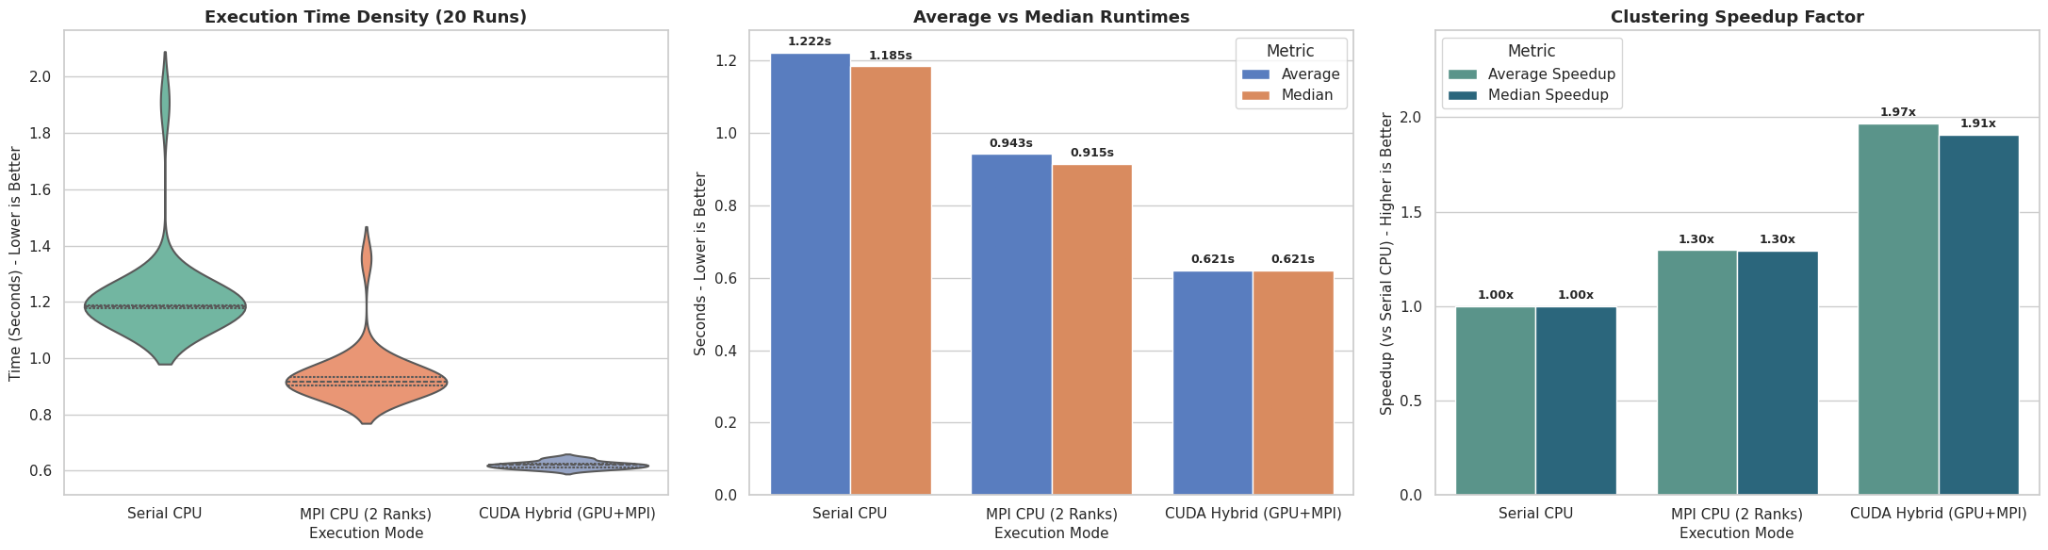
\includegraphics[width=\textwidth]{kmeans_performance.png}
\caption{Runtime distributions over 20 runs, mean and median runtimes, and speedup relative to the serial CPU baseline.}
\label{fig:performance}
\end{figure*}

CUDA Hybrid is the fastest mode in this experiment. Its mean runtime is about 49.2\% lower than the serial result, while two-rank MPI reduces the mean by about 22.8\%. These percentages apply to the stated dataset and test environment; they should not be assumed to hold for other problem sizes or hardware.

\subsection{Execution screenshots}
The benchmark plot was provided, but terminal screenshots for the three program runs were not available in the materials used to prepare this report. Replace each placeholder below with a screenshot captured from the corresponding run before submission. The source file will include images saved under the filenames shown in the panels.



% ------------------------------------------------------------------
\section{Performance Analysis}
\label{sec:performance}
Speedup is the serial runtime divided by the runtime of the selected parallel version. For mean runtimes, it is
\begin{equation}
S_{\mathrm{mean}}=\frac{T_{\mathrm{serial,mean}}}{T_{\mathrm{mode,mean}}}.
\end{equation}
For two-rank MPI, the conventional efficiency estimate is $E=S/P$, with $P=2$. The mean values give $S=1.222/0.943\approx1.297$, so the estimated efficiency is $1.297/2\approx64.8\%$. The median values give $1.185/0.915\approx1.295$, which leads to nearly the same estimate. Since these calculations use end-to-end runtime, communication and other implementation costs are included.

The hybrid result is reported as speedup rather than rank-based efficiency. A CPU rank and a GPU are not equivalent processing units, and the graph does not provide enough information to define a comparable processor count. The end-to-end speedup against the serial program remains meaningful for this workload.

The violin plot places most CUDA Hybrid runs close to 0.62 s. The CPU distributions are wider, and the serial results include a small number of slower runs. The figure does not provide the raw timings, so standard deviation, confidence intervals, and exact outlier counts cannot be calculated from it.

\subsection{Strong scaling}
Strong scaling measures how runtime changes as more processing elements work on a fixed problem. For this workload, a fuller test would keep $N=100{,}000$, $D=16$, and $K=10$ constant while measuring several MPI sizes, for example $P\in\{1,2,4,8\}$. The current results contain only the serial baseline and one two-rank MPI measurement, so they do not establish a strong-scaling curve.

\subsection{Weak scaling}
Weak scaling keeps the amount of work per rank approximately constant as more ranks are added. One way to test it is to increase $N$ with $P$ while keeping $D$, $K$, and the data-generation procedure fixed. Since the current chart uses one problem size, it provides no weak-scaling measurement.

\subsection{Limitations affecting performance}
The timing includes per-iteration allocation and data transfers, so it measures more than kernel work. Global-memory atomics may also limit cluster accumulation, particularly when several MPI ranks share a GPU. Empty clusters are left unchanged. These costs should be kept in mind when reading the results.

% ------------------------------------------------------------------
\section{Comparison with Existing Methods}
\label{sec:comparison}
The runtime table compares the serial implementation with two parallel variants under the same workload. Serial K-means is straightforward and avoids communication, but all distance calculations run on the CPU. MPI distributes those calculations across two ranks and reduces the mean runtime by 22.8\%. The hybrid version records the lowest mean runtime, with a reduction of 49.2\% against the serial baseline.

Prior work has also studied distributed-memory and GPU-based K-means \cite{dhillon2000,farivar2008,li2013}. A numerical comparison with those papers would require matching the processor and GPU models, dataset, cluster count, initialization, stopping condition, and timing method. The present results should therefore be read as a comparison among the three implementations in this project, not as a claim that they outperform published systems in general.

% ------------------------------------------------------------------
\section{Conclusion}
\label{sec:conclusion}
This project implements the Lloyd iteration of K-means in three forms: serial CPU, two-rank MPI CPU, and hybrid MPI+CUDA. The MPI program distributes points and combines local cluster statistics at each iteration. The hybrid version replaces the local CPU assignment with a CUDA kernel and uses the CPU routine if a usable device is unavailable. A shared numerical interface makes it possible to compare the versions using the same input and validation checks.

For the workload of 100,000 points, 16 features, and 10 clusters, CUDA Hybrid records a mean runtime of 0.621 s, compared with 0.943 s for MPI CPU and 1.222 s for Serial CPU. These measurements correspond to mean speedups of about $1.97\times$ for the hybrid version and $1.30\times$ for MPI. The estimated efficiency of the two-rank MPI run is 64.8\%. Additional tests at other rank counts and data sizes are needed before drawing broader conclusions about scalability.

% ------------------------------------------------------------------
\section{Future Scope}
\label{sec:future}
The next evaluation should retain the raw timing data and record the complete hardware and software configuration. Strong-scaling tests can hold the dataset fixed while varying the MPI rank count. Weak-scaling tests can increase the point count in proportion to the number of ranks. Each case should be repeated and reported with measures of spread, not only the mean and median.

Several code changes are also worth measuring. Reusing device buffers across iterations would avoid repeated allocation. Profiling could separate data-transfer time from kernel time, while block-level accumulation may reduce pressure on global atomics. The implementation could also add a policy for empty clusters and compare uniform sampling with K-means++ initialization. Each change should pass the existing SSE and centroid-matching checks before its timing results are considered.

% ------------------------------------------------------------------
\begin{thebibliography}{99}
\bibitem{macqueen1967}
J.~MacQueen.
\newblock Some methods for classification and analysis of multivariate observations.
\newblock In \emph{Proceedings of the Fifth Berkeley Symposium on Mathematical Statistics and Probability}, volume~1, pages 281--297, 1967.
\bibitem{lloyd1982}
S.~P. Lloyd.
\newblock Least squares quantization in PCM.
\newblock \emph{IEEE Transactions on Information Theory}, 28(2):129--137, 1982.
\bibitem{dhillon2000}
I.~S. Dhillon and D.~S. Modha.
\newblock A data-clustering algorithm on distributed memory multiprocessors.
\newblock In \emph{Large-Scale Parallel Data Mining}, Lecture Notes in Computer Science, volume 1759, pages 245--260. Springer, 2000.
\bibitem{farivar2008}
R.~Farivar, D.~Rebolledo, E.~Chan, and R.~Campbell.
\newblock A parallel implementation of $K$-means clustering on GPUs.
\newblock In \emph{Proceedings of the International Conference on Parallel and Distributed Processing Techniques and Applications (PDPTA)}, pages 340--345, 2008.
\bibitem{li2013}
Y.~Li, K.~Zhao, X.~Chu, and J.~Liu.
\newblock Speeding up $k$-means algorithm by GPUs.
\newblock \emph{Journal of Computer and System Sciences}, 79(2):216--229, 2013.
\bibitem{arthur2007}
D.~Arthur and S.~Vassilvitskii.
\newblock $k$-means++: The advantages of careful seeding.
\newblock In \emph{Proceedings of the Eighteenth Annual ACM-SIAM Symposium on Discrete Algorithms (SODA)}, pages 1027--1035, 2007.
\bibitem{mpi40}
Message Passing Interface Forum.
\newblock \emph{MPI: A Message-Passing Interface Standard, Version 4.1}, 2023.
\bibitem{lecun-mnist}
Y.~LeCun, C.~Cortes, and C.~J.~C. Burges.
\newblock The MNIST database of handwritten digits.
\newblock \url{http://yann.lecun.com/exdb/mnist/}.
\bibitem{kddcup1999}
S.~Stolfo, W.~Fan, W.~Lee, A.~Prodromidis, and P.~Chan.
\newblock KDD Cup 1999 Data.
\newblock UCI Machine Learning Repository, 1999.
\bibitem{census1990}
C.~Meek, B.~Thiesson, and D.~Heckerman.
\newblock US Census Data (1990).
\newblock UCI Machine Learning Repository, 2001.
\end{thebibliography}
\newpage
\section*{Plagiarism Check}
\begin{figure}[!ht]
  \centering
  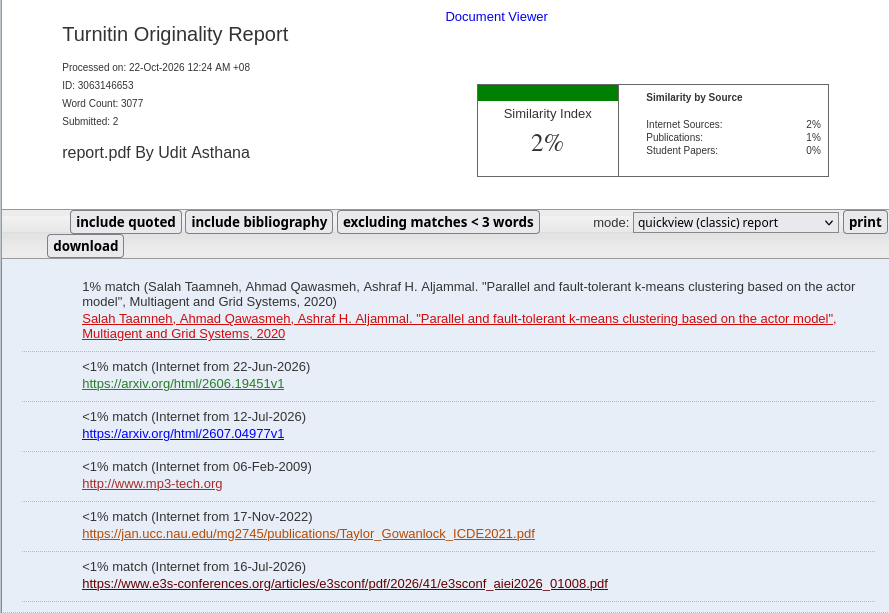
\includegraphics[width=\textwidth,height=0.88\textheight,keepaspectratio]{turnitin-plag-check.png}
  \caption{The turnitin Plagiarism check. Shows $2\%$ similarity.}
\end{figure}
\end{document}
\end{document}
